\documentclass[aspectratio=169,12pt,handout]{beamer}
\usepackage{pgfpages}
\pgfpagesuselayout{resize to}[letterpaper,landscape,border shrink=5mm]
\usetheme{Madrid}
\usecolortheme{default}
\usepackage{graphicx}
\usepackage{booktabs}
\usepackage{amsmath}

% Clean colors
\definecolor{binggreen}{RGB}{0,100,0}
\setbeamercolor{structure}{fg=binggreen}
\setbeamercolor{title}{fg=white,bg=binggreen}
\setbeamercolor{frametitle}{fg=white,bg=binggreen}

\setbeamertemplate{navigation symbols}{}
\setbeamertemplate{footline}{%
  \hfill\insertframenumber/\inserttotalframenumber\hspace{2mm}\vspace{2mm}%
}

\hypersetup{pdfpagelayout=SinglePage}

\title{Method Gating \& Visual Similarity}
\subtitle{Week of April 16}
\author{}
\institute{Binghamton University}
\date{April 2026}

\begin{document}

% ------------------------------------------------------------------
\begin{frame}
\titlepage
\end{frame}

% ------------------------------------------------------------------
\begin{frame}{Problem: Some Methods Pick the Wrong Genes}
\begin{columns}[T]
\begin{column}{0.55\textwidth}
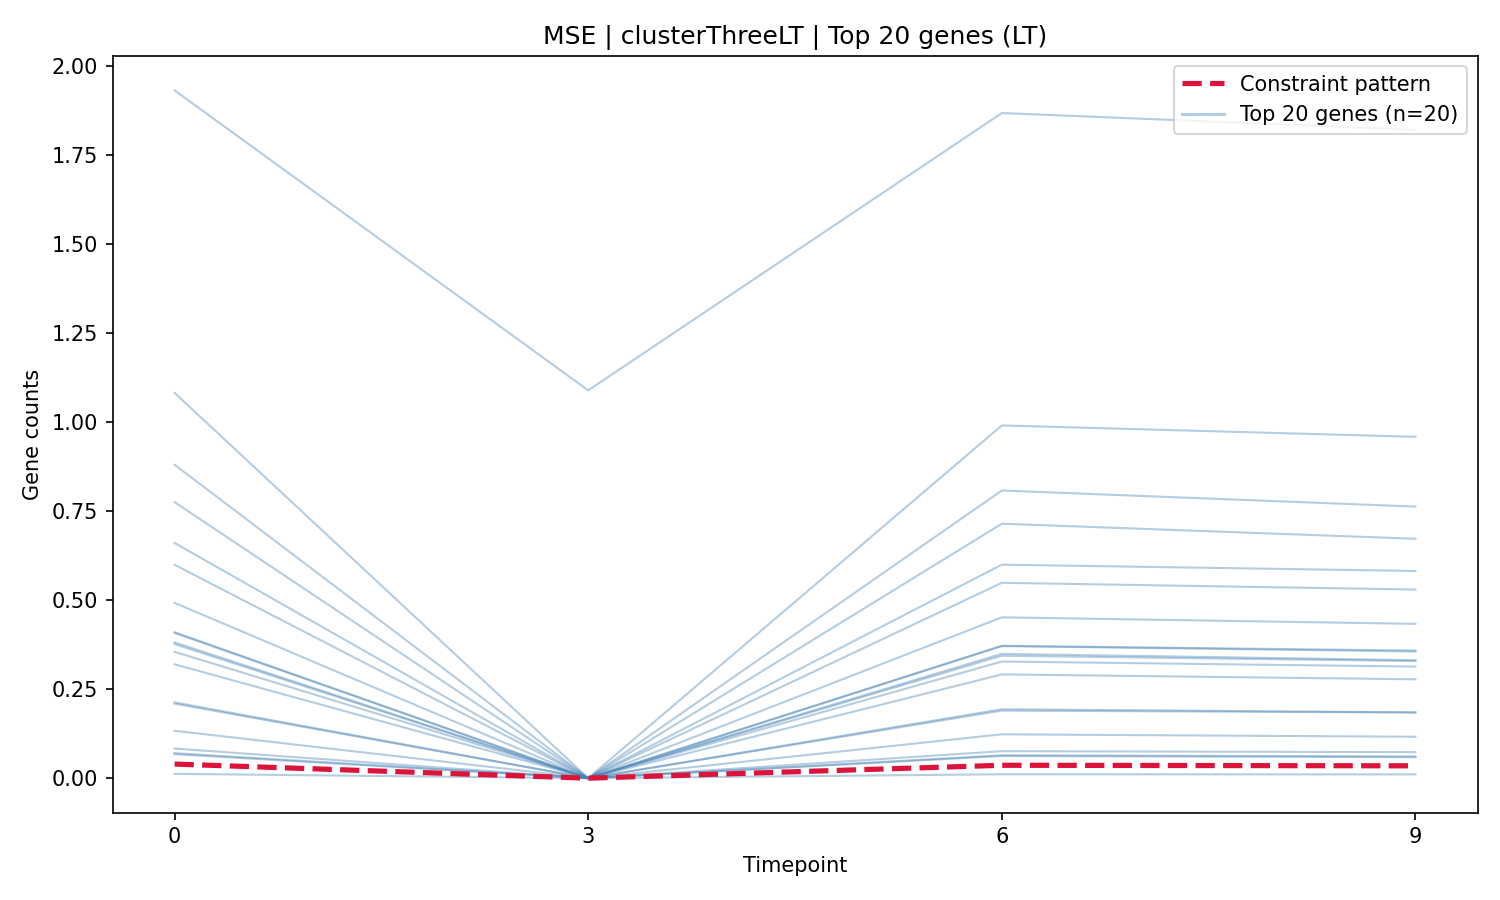
\includegraphics[width=\textwidth]{../Week of April 9th/plots/MSE_LT_clusterThreeLT_constraint.png}
\end{column}
\begin{column}{0.42\textwidth}
\vspace{1em}
\textbf{MSE on clusterThree LT}\\[0.5em]
Top-20 genes are scattered far above the constraint pattern (red dashed).\\[0.5em]
MSE finds genes that are close on \textit{normalized} data, but at completely different expression levels in reality.
\end{column}
\end{columns}
\end{frame}

% ------------------------------------------------------------------
\begin{frame}{Problem: Some Methods Pick the Wrong Genes}
\begin{columns}[T]
\begin{column}{0.55\textwidth}
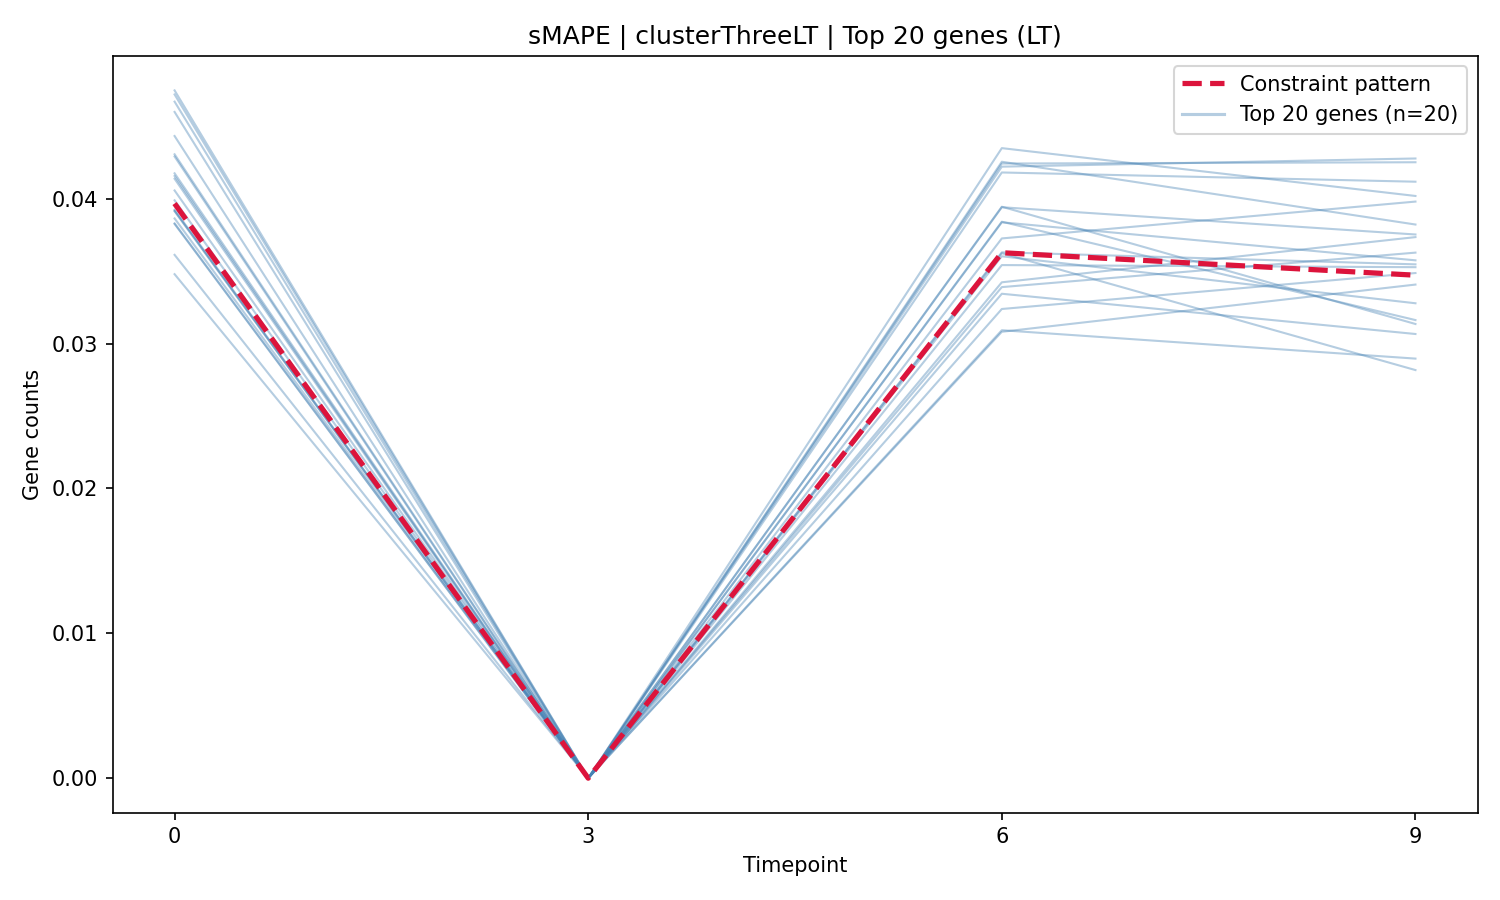
\includegraphics[width=\textwidth]{../Week of April 9th/plots/sMAPE_LT_clusterThreeLT_constraint.png}
\end{column}
\begin{column}{0.42\textwidth}
\vspace{1em}
\textbf{sMAPE on clusterThree LT}\\[0.5em]
Top-20 genes tightly follow the constraint pattern.\\[0.5em]
Same cluster, same pattern --- but only sMAPE finds the right genes.\\[0.5em]
\textbf{Can we automatically detect when a method isn't working?}
\end{column}
\end{columns}
\end{frame}

% ------------------------------------------------------------------
\begin{frame}{Attempt 1: Fixed Score Thresholds}
\begin{columns}[T]
\begin{column}{0.55\textwidth}
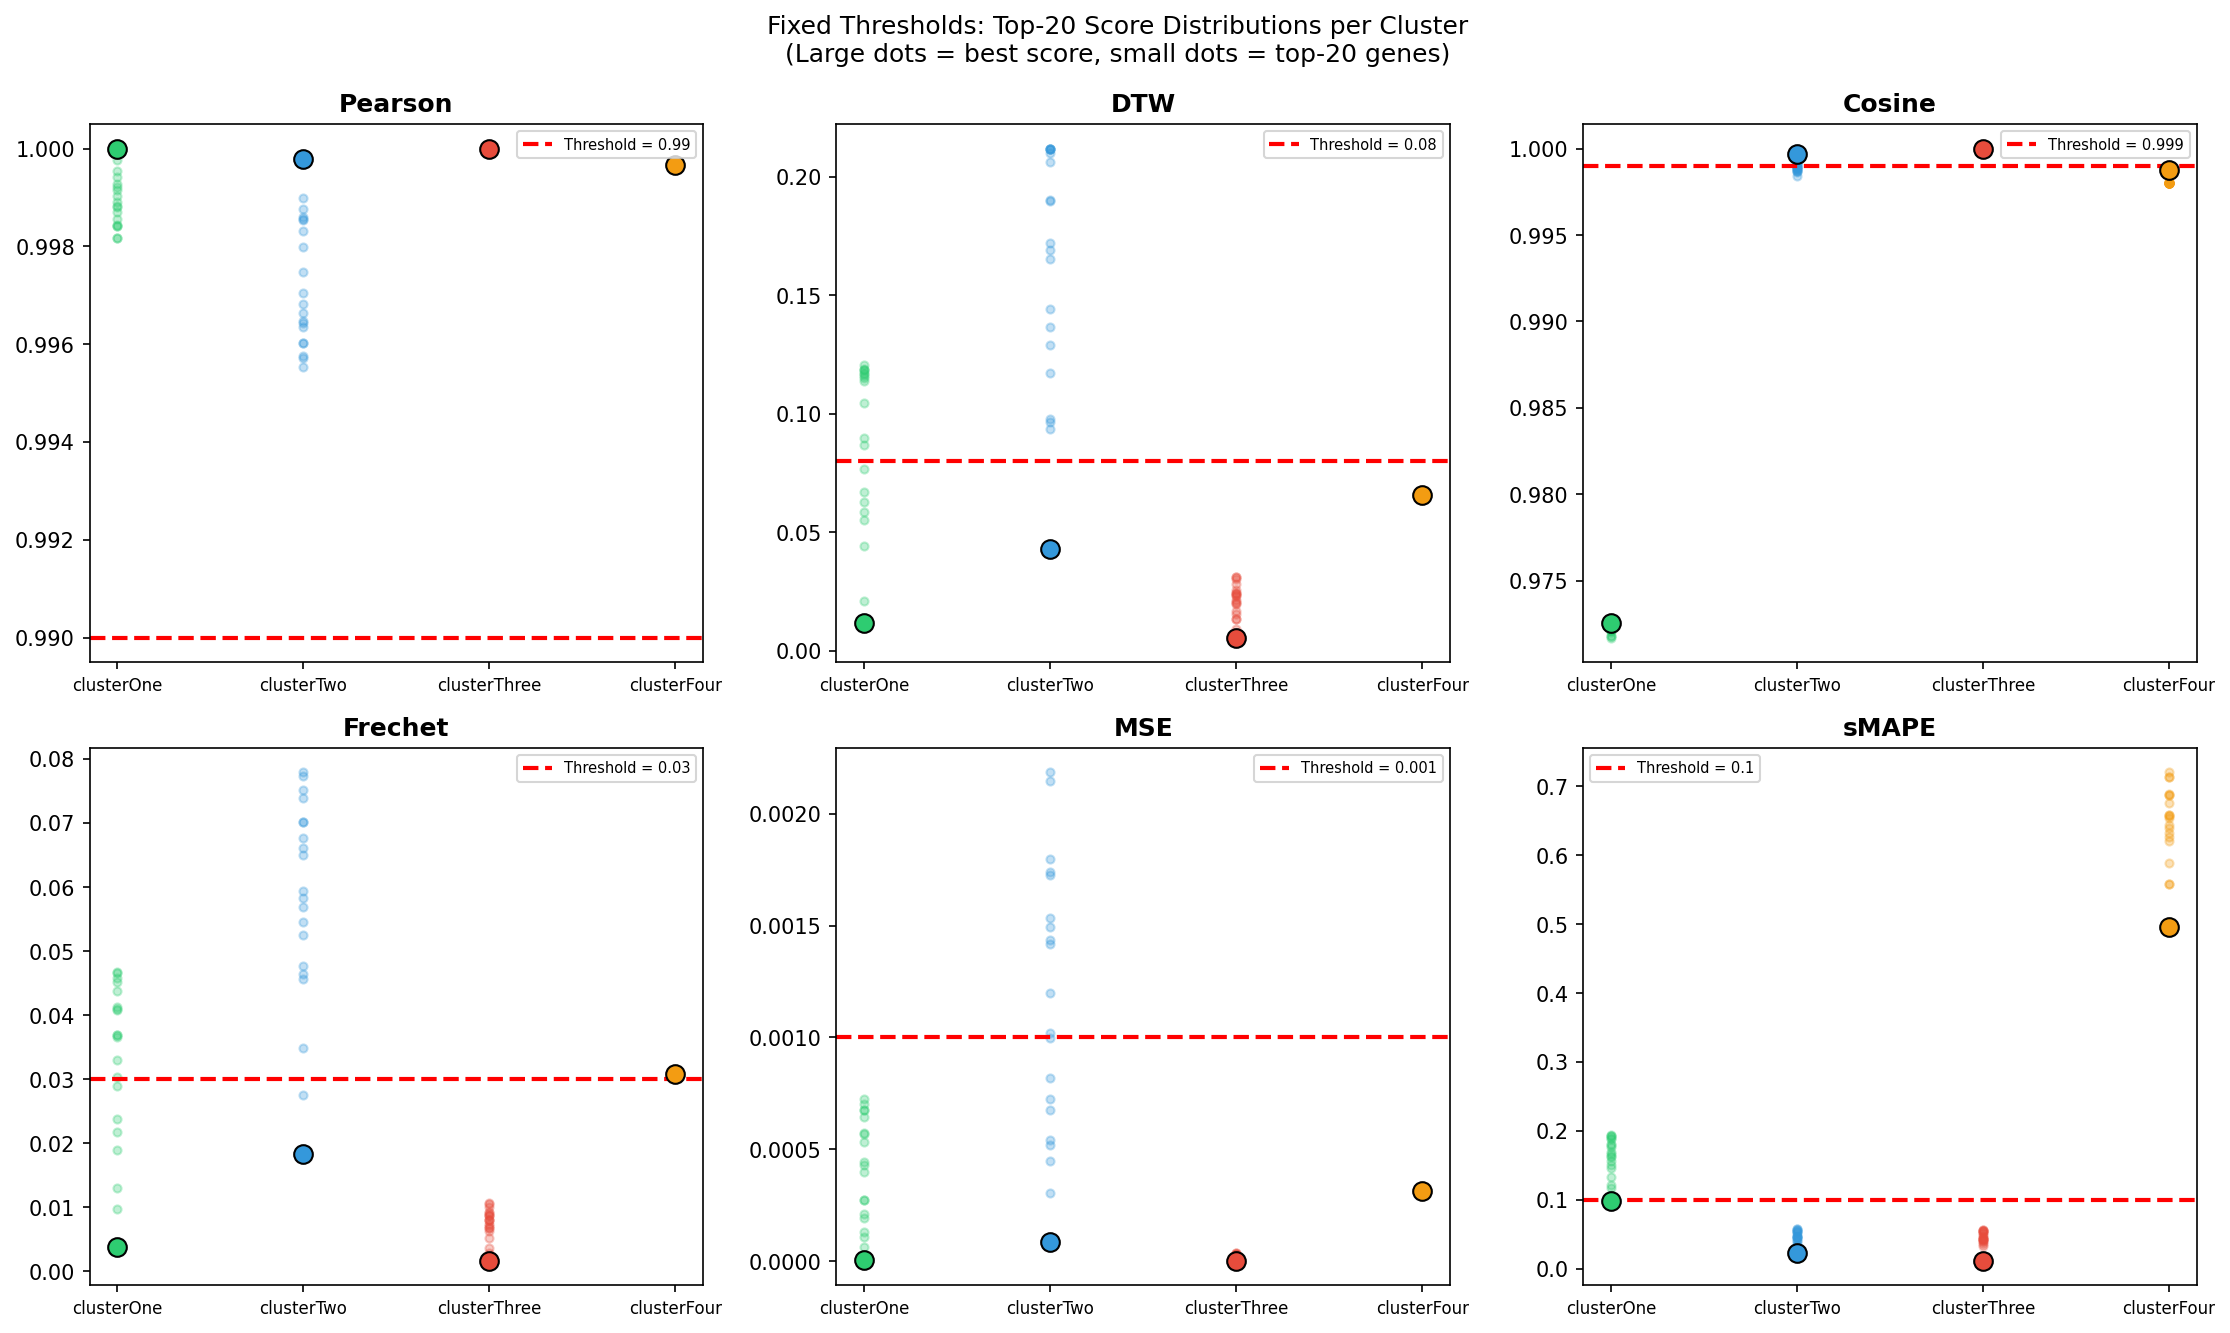
\includegraphics[width=\textwidth]{plots/act1_threshold_sweep.png}
\end{column}
\begin{column}{0.42\textwidth}
\vspace{0.5em}
\textbf{Idea:} Set a quality floor on each metric's score. If a method's best genes don't meet it, the method can't vote.\\[0.5em]
Each subplot shows one method's top-20 scores across 4 clusters. The red line is the threshold.\\[0.5em]
\textbf{Problem:} The same method has very different score ranges across clusters --- no single line works.
\end{column}
\end{columns}
\end{frame}

% ------------------------------------------------------------------
\begin{frame}{What If We Force the ``Right'' Answer?}
\begin{columns}[T]
\begin{column}{0.55\textwidth}
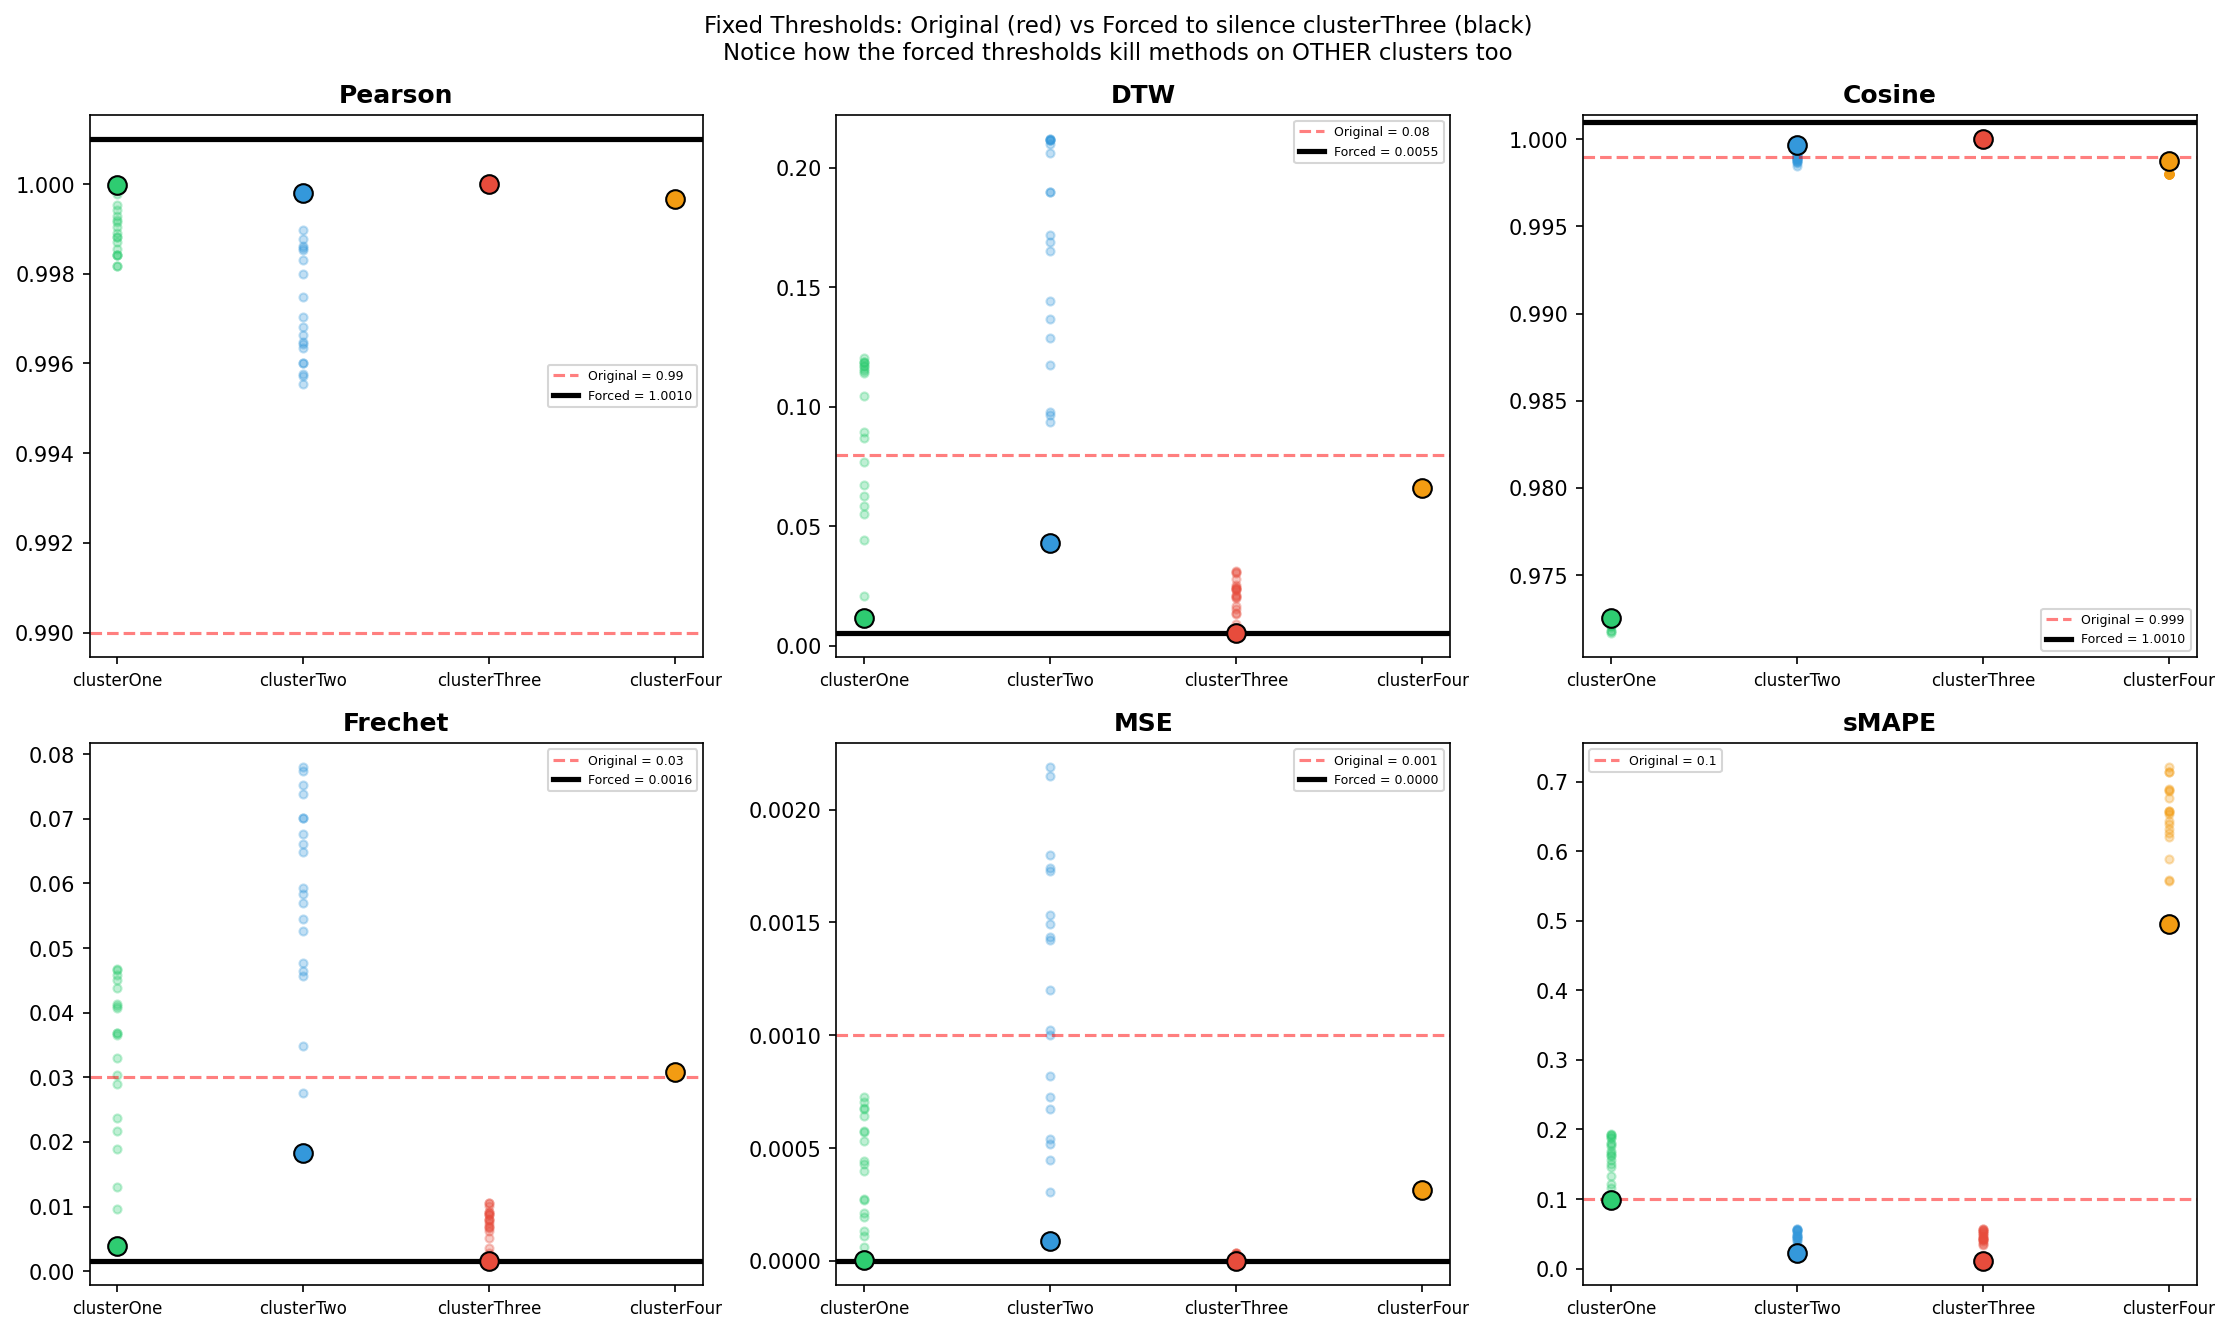
\includegraphics[width=\textwidth]{plots/act1_forced_thresholds.png}
\end{column}
\begin{column}{0.42\textwidth}
\vspace{0.5em}
Since sMAPE is the only method that visually works on clusterThree, what thresholds would we need to silence everything else there?\\[0.5em]
Black lines = forced thresholds.\\
Red lines = original thresholds.\\[0.5em]
The forced thresholds are so extreme they cut through \textit{every} cluster's scores.
\end{column}
\end{columns}
\end{frame}

% ------------------------------------------------------------------
\begin{frame}{Forced Thresholds: Collateral Damage}
\begin{center}
\large
To silence non-sMAPE methods on clusterThree:\\[0.5em]
\begin{tabular}{lll}
\toprule
\textbf{Method} & \textbf{Original} & \textbf{Required} \\
\midrule
Pearson & $> 0.99$ & $> 1.001$ (impossible) \\
DTW & $< 0.08$ & $< 0.006$ \\
MSE & $< 0.001$ & $< 0.000001$ \\
\bottomrule
\end{tabular}

\vspace{1em}
\textbf{Result:} Every method silenced on every cluster\\
except sMAPE --- which only survives on 3 of 4 clusters.\\[0.5em]
\normalsize
Fixed thresholds can't work because the methods are actually\\
\textit{confident} on clusterThree (Pearson $= 1.0$) --- just about the wrong genes.
\end{center}
\end{frame}

% ------------------------------------------------------------------
\begin{frame}{Why Are the Methods So Confident on the Wrong Genes?}
\begin{center}
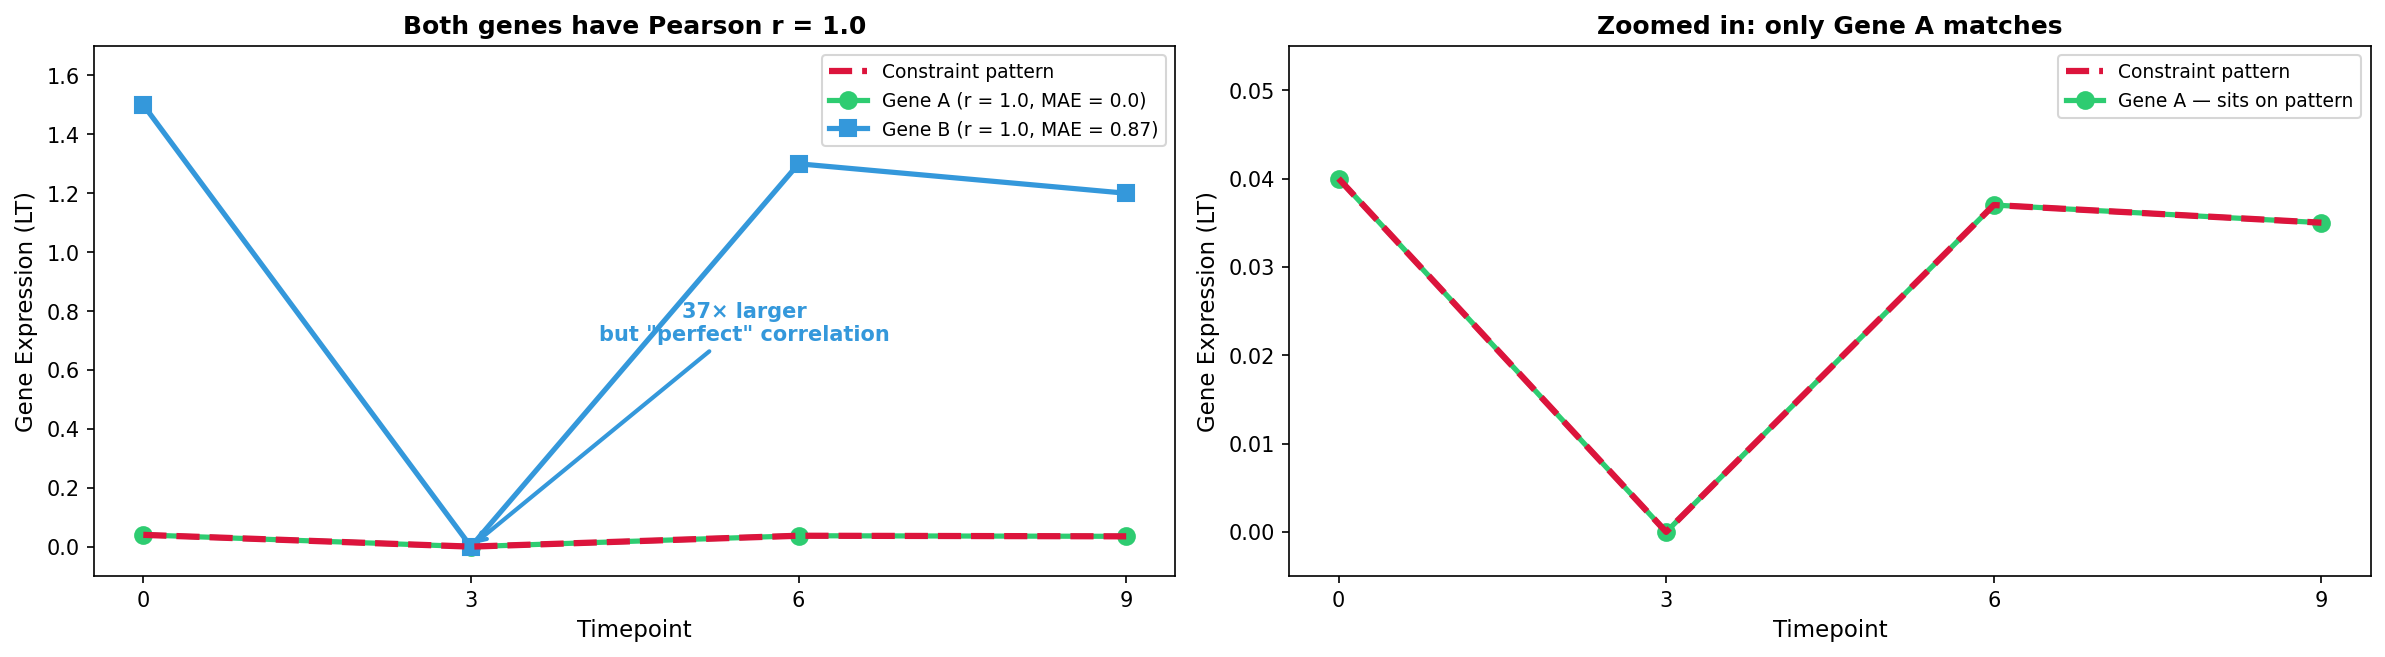
\includegraphics[width=\textwidth]{plots/pearson_visual_explanation.png}
\end{center}
\vspace{-0.5em}
\small\centering
Gene B (blue) is 37$\times$ larger than the pattern, but both have Pearson $r = 1.0$.\\
On the plot Gene A (green) sits on the pattern; Gene B is nowhere near it.
\end{frame}

% ------------------------------------------------------------------
\begin{frame}{Why Pearson $= 1.0$: Step-by-Step}
\small
\textbf{Step 1:} Pearson subtracts each series' mean before comparing.
\quad Gene B mean $= 1.0$, \quad Pattern mean $= 0.028$

\vspace{0.3em}
\textbf{Step 2:} After subtracting means, the residuals are:
\begin{center}
\begin{tabular}{l cccc}
\toprule
 & $t=0$ & $t=3$ & $t=6$ & $t=9$ \\
\midrule
Gene B residual & $+0.50$ & $-1.00$ & $+0.30$ & $+0.20$ \\
Pattern residual & $+0.012$ & $-0.028$ & $+0.009$ & $+0.007$ \\
\midrule
Same sign? & \textcolor{binggreen}{\checkmark\; +/+} & \textcolor{binggreen}{\checkmark\; $-$/$-$} & \textcolor{binggreen}{\checkmark\; +/+} & \textcolor{binggreen}{\checkmark\; +/+} \\
\bottomrule
\end{tabular}
\end{center}

\vspace{0.3em}
\textbf{Step 3:} Pearson multiplies the residuals at each timepoint:
\begin{center}
\begin{tabular}{lcccc l}
 & $t=0$ & $t=3$ & $t=6$ & $t=9$ & \\
\midrule
product & $(+)(+)$ & $(-)(-)$ & $(+)(+)$ & $(+)(+)$ & \\
 & $= +0.006$ & $= +0.028$ & $= +0.003$ & $= +0.001$ & sum $= +0.038$ \\
\end{tabular}
\end{center}

\vspace{0.3em}
\textbf{Every product is positive} because the signs always match.\\
The denominator just rescales to $[-1, 1]$: \quad $r = 0.038\; /\; 0.038 = \mathbf{1.0}$\\[0.3em]
\centering
\textbf{Gene B is 37$\times$ larger, but the ups and downs match --- so $r$ is perfect.}
\end{frame}

% ------------------------------------------------------------------
\begin{frame}{Attempt 2: Data-Driven Gating}
\begin{itemize}\itemsep6pt
  \item Fixed thresholds fail because the methods' own scores can't distinguish
        ``confident and right'' from ``confident and wrong''
  \item \textbf{New idea:} check whether a method's top genes actually sit near the
        pattern in expression space
  \item For each method $\times$ cluster: average the top-20 genes into a centroid,
        then measure how far that centroid is from the pattern
  \item Normalize by pattern range so scores are comparable across clusters:
\end{itemize}
\[\text{Relative Centroid Error} = \frac{\text{MSE}(\bar{x}_{\text{top-20}},\; p)}{(\max p - \min p)^2}\]
\begin{itemize}
  \item One universal cutoff applied everywhere $\rightarrow$ methods with high error are silenced
\end{itemize}
\end{frame}

% ------------------------------------------------------------------
\begin{frame}{Gated Results: clusterThree (1/6 methods active --- sMAPE only)}
\begin{columns}[T]
\begin{column}{0.58\textwidth}
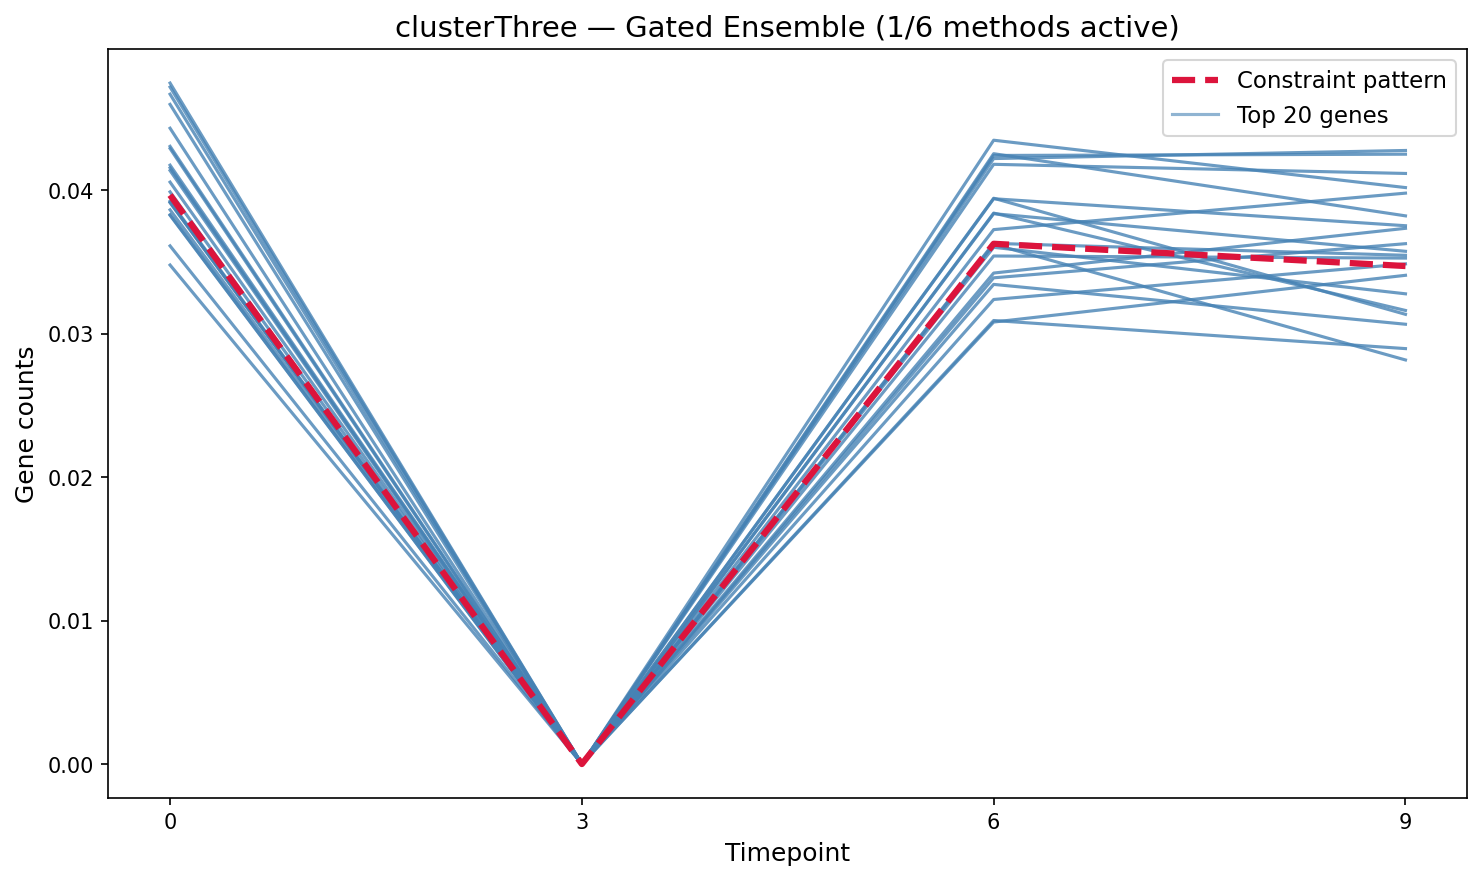
\includegraphics[width=\textwidth]{plots/gated_clusterThree.png}
\end{column}
\begin{column}{0.40\textwidth}
\vspace{1em}
The gate correctly silences all methods except sMAPE on clusterThree.\\[0.5em]
sMAPE's centroid error: \textbf{0.001}\\
Other methods: 41--80\\[0.5em]
This matches exactly what we'd pick visually.
\end{column}
\end{columns}
\end{frame}

% ------------------------------------------------------------------
\begin{frame}{Gated Results: clusterTwo (6/6 methods active)}
\begin{columns}[T]
\begin{column}{0.58\textwidth}
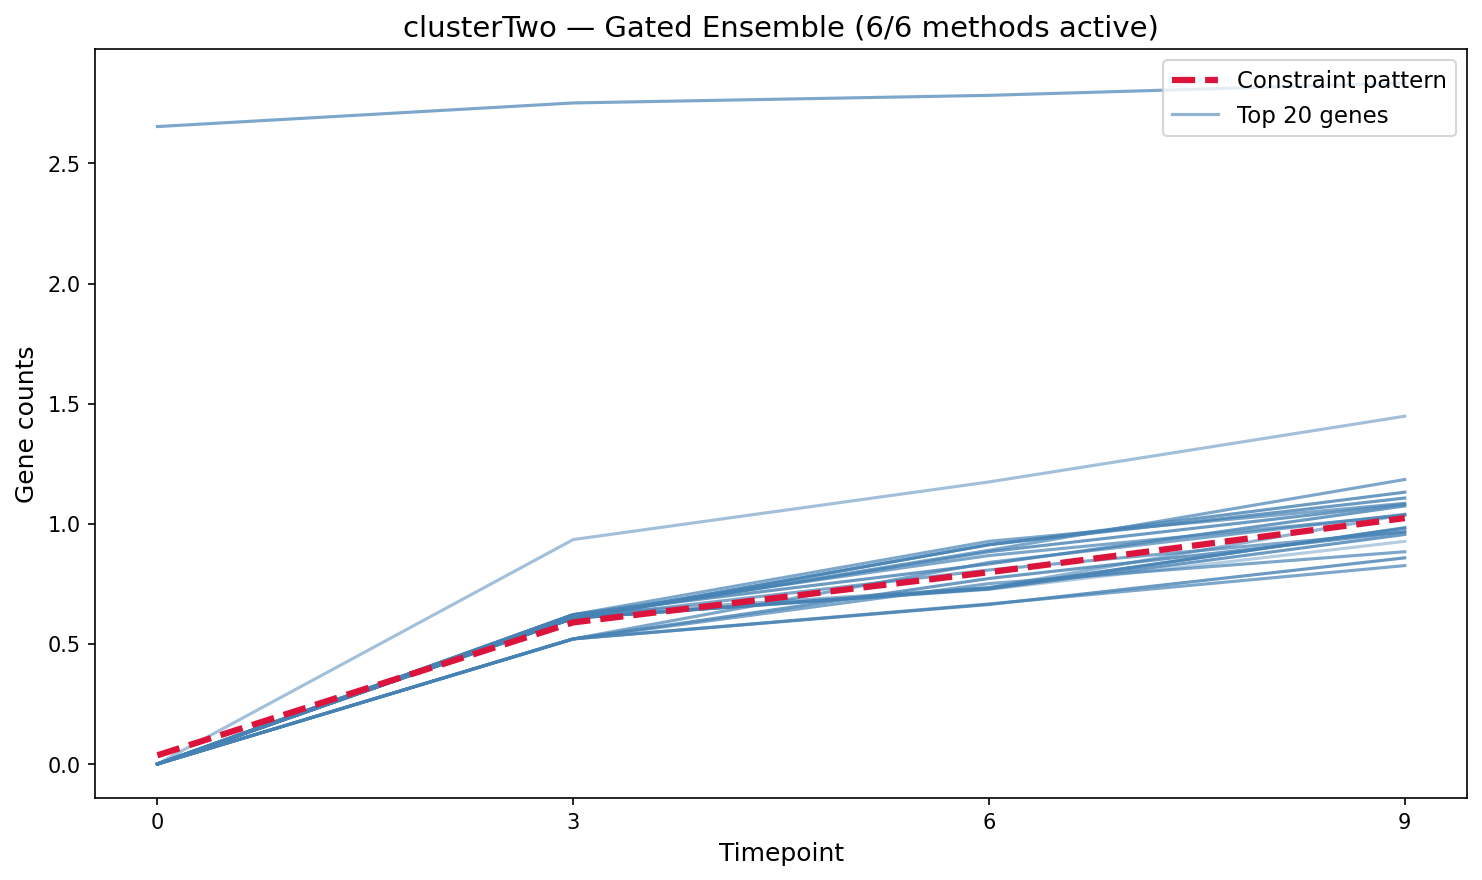
\includegraphics[width=\textwidth]{plots/gated_clusterTwo.png}
\end{column}
\begin{column}{0.40\textwidth}
\vspace{1em}
All 6 methods pass the gate --- their top genes genuinely sit near the pattern.\\[0.5em]
The gate correctly does \textit{not} silence methods where they all work.\\[0.5em]
Same consensus genes as before (RAB14, SYNGR1, etc. at 6/6 unanimous).
\end{column}
\end{columns}
\end{frame}

% ------------------------------------------------------------------
\begin{frame}{But: Gated clusterOne and clusterFour Still Don't Fit}
\begin{columns}[T]
\begin{column}{0.48\textwidth}
\centering
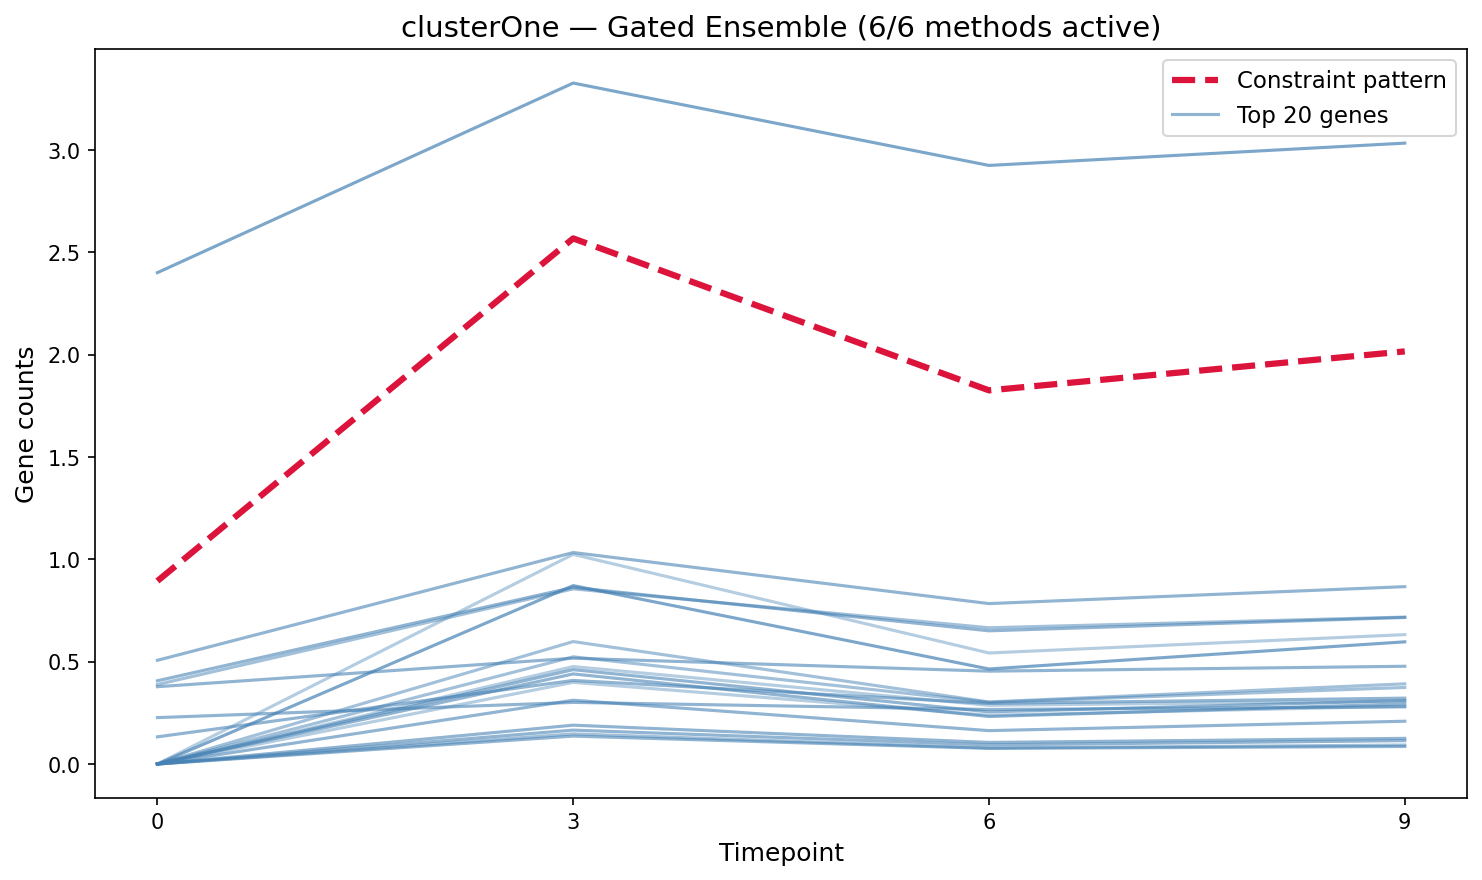
\includegraphics[width=\textwidth]{plots/gated_clusterOne.png}\\
\small Genes follow the shape but\\sit below the pattern
\end{column}
\begin{column}{0.48\textwidth}
\centering
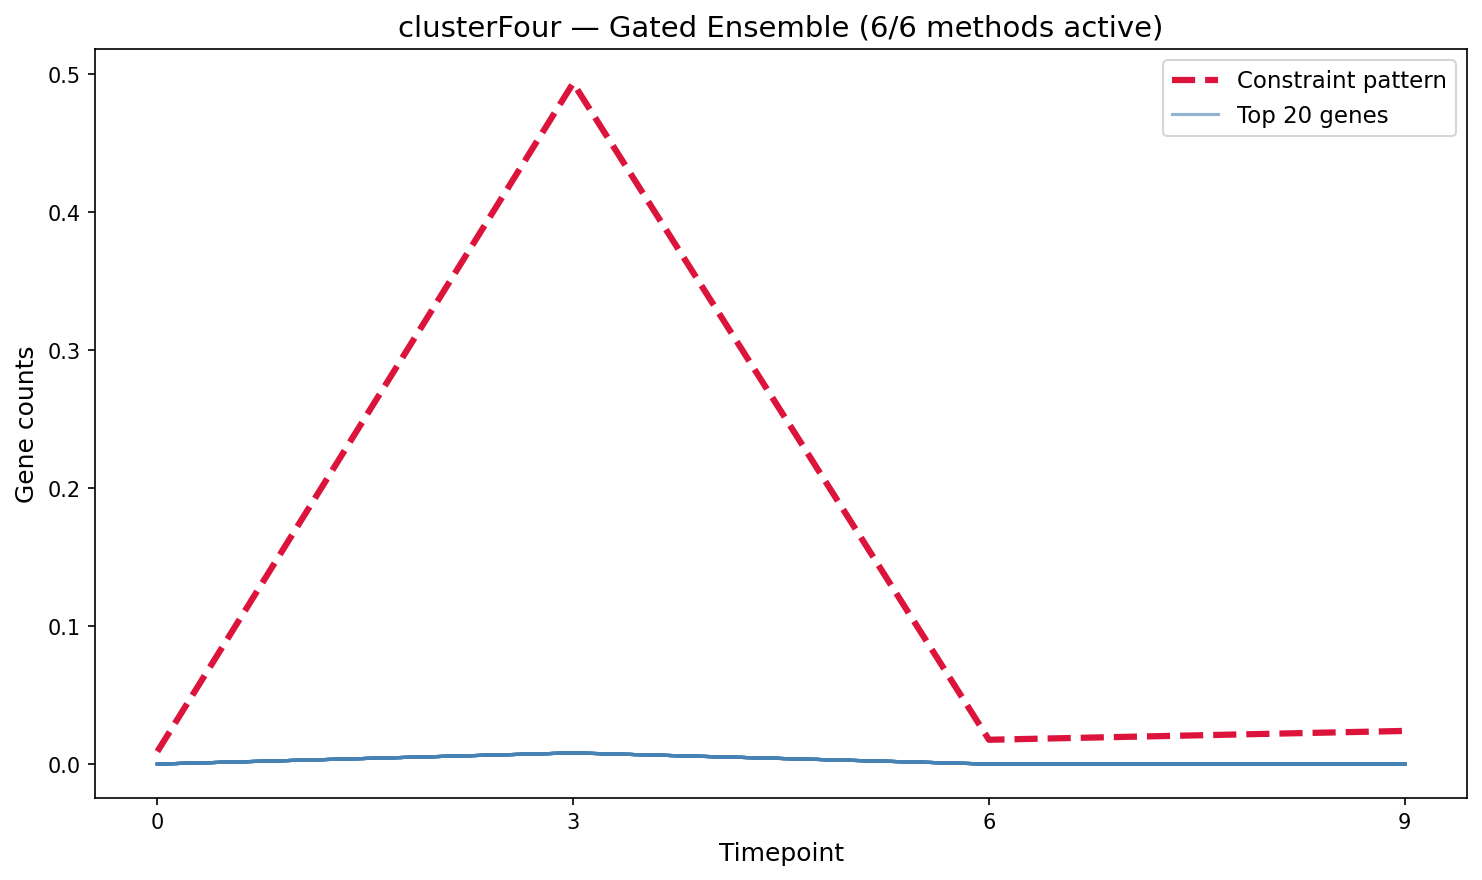
\includegraphics[width=\textwidth]{plots/gated_clusterFour.png}\\
\small 6/6 active but genes are flat ---\\nothing matches the spike
\end{column}
\end{columns}
\vspace{0.5em}
\centering
\small The gate checks if top genes are near the pattern \textit{relative to its range} --- so these pass because the centroid error is small \textit{as a proportion}. But the genes are still far from the pattern in \textbf{absolute} terms. The root cause: all 6 methods operate on \textbf{normalized} data, which erases magnitude before scoring. Can we do better?
\end{frame}

% ------------------------------------------------------------------
\begin{frame}{A Simpler Idea: Raw-Space MAE}
\begin{center}
\large
All 6 methods work on \textbf{normalized} data ---\\
so they find genes with the right \textit{shape} but at any magnitude.\\[0.8em]
What if we skip normalization entirely?\\[0.5em]
$\text{MAE} = \frac{1}{4}\sum_{t} |g_t - p_t|$\\[0.8em]
\normalsize
No normalization. No correlation. No gating needed.\\[0.3em]
Just rank all 17,856 genes by how close they are\\
to the pattern \textbf{in the actual expression space}.
\end{center}
\end{frame}

% ------------------------------------------------------------------
\begin{frame}{Raw MAE: clusterTwo}
\begin{columns}[T]
\begin{column}{0.62\textwidth}
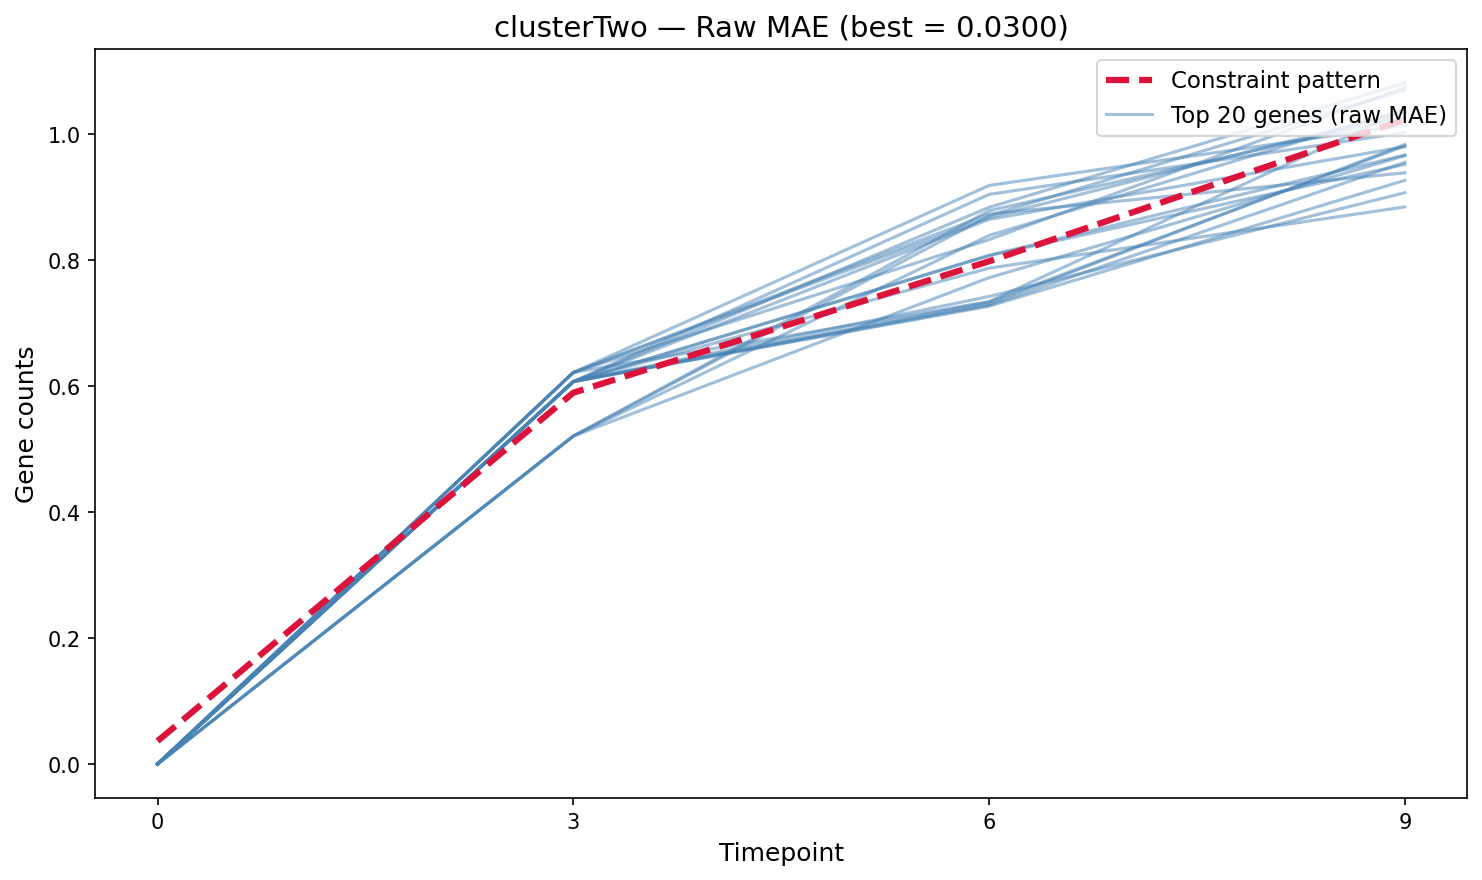
\includegraphics[width=\textwidth]{plots/rawmae_clusterTwo.png}
\end{column}
\begin{column}{0.36\textwidth}
\vspace{1em}
Genes tightly follow the steady-increase pattern.\\[0.5em]
8--12/20 overlap with all 6 original methods --- confirming the existing consensus.
\end{column}
\end{columns}
\end{frame}

% ------------------------------------------------------------------
\begin{frame}{Raw MAE: clusterThree}
\begin{columns}[T]
\begin{column}{0.62\textwidth}
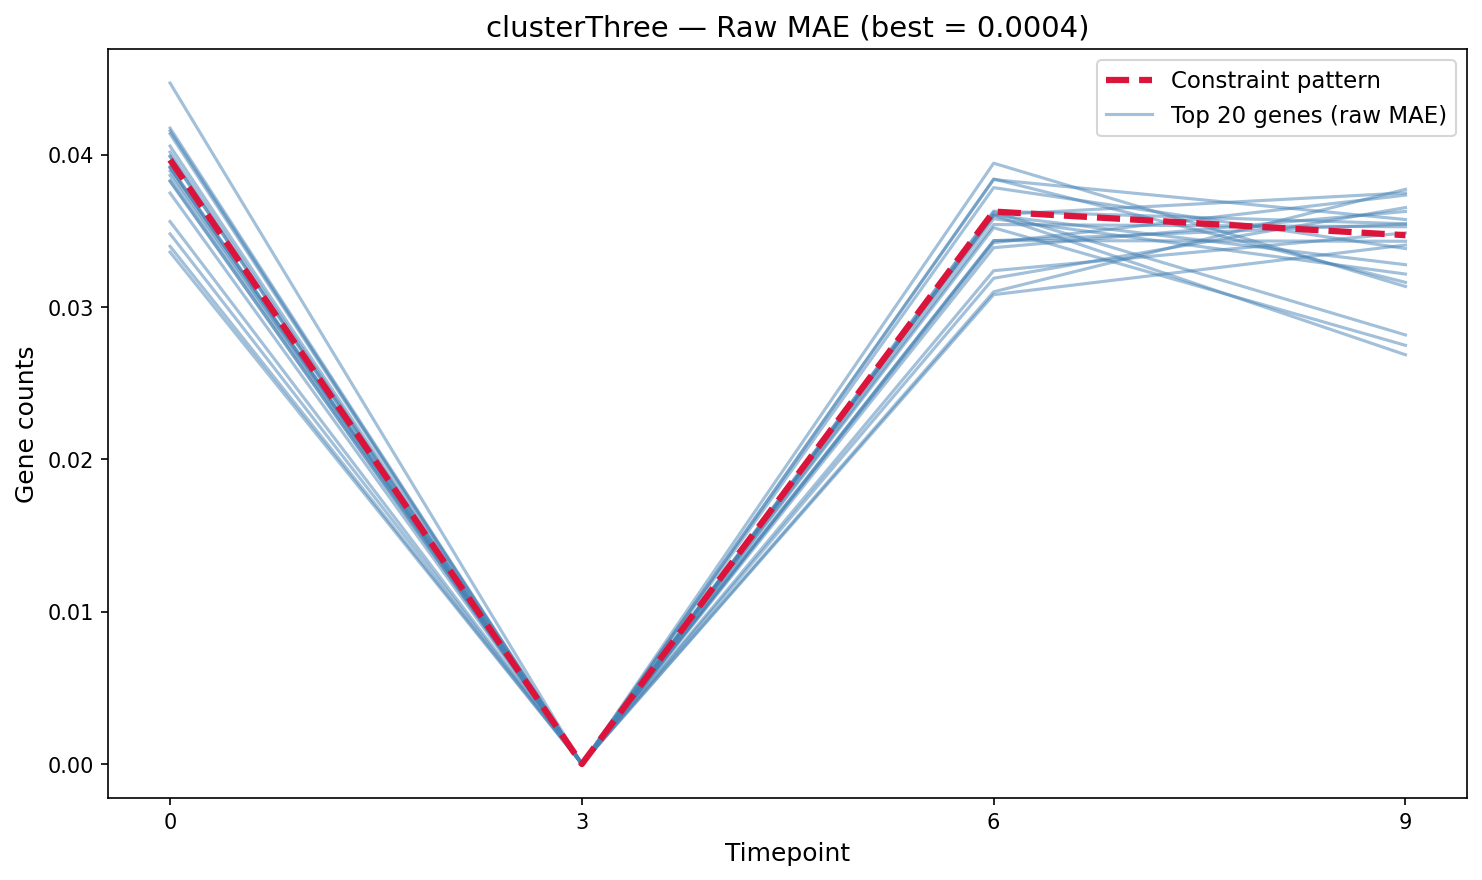
\includegraphics[width=\textwidth]{plots/rawmae_clusterThree.png}
\end{column}
\begin{column}{0.36\textwidth}
\vspace{1em}
Genes sit right on the pattern.\\[0.5em]
11/20 overlap with sMAPE,\\
0/20 with all other methods.\\[0.5em]
Raw MAE independently confirms sMAPE was the only method finding the right genes.
\end{column}
\end{columns}
\end{frame}

% ------------------------------------------------------------------
\begin{frame}{Raw MAE: clusterFour}
\begin{columns}[T]
\begin{column}{0.62\textwidth}
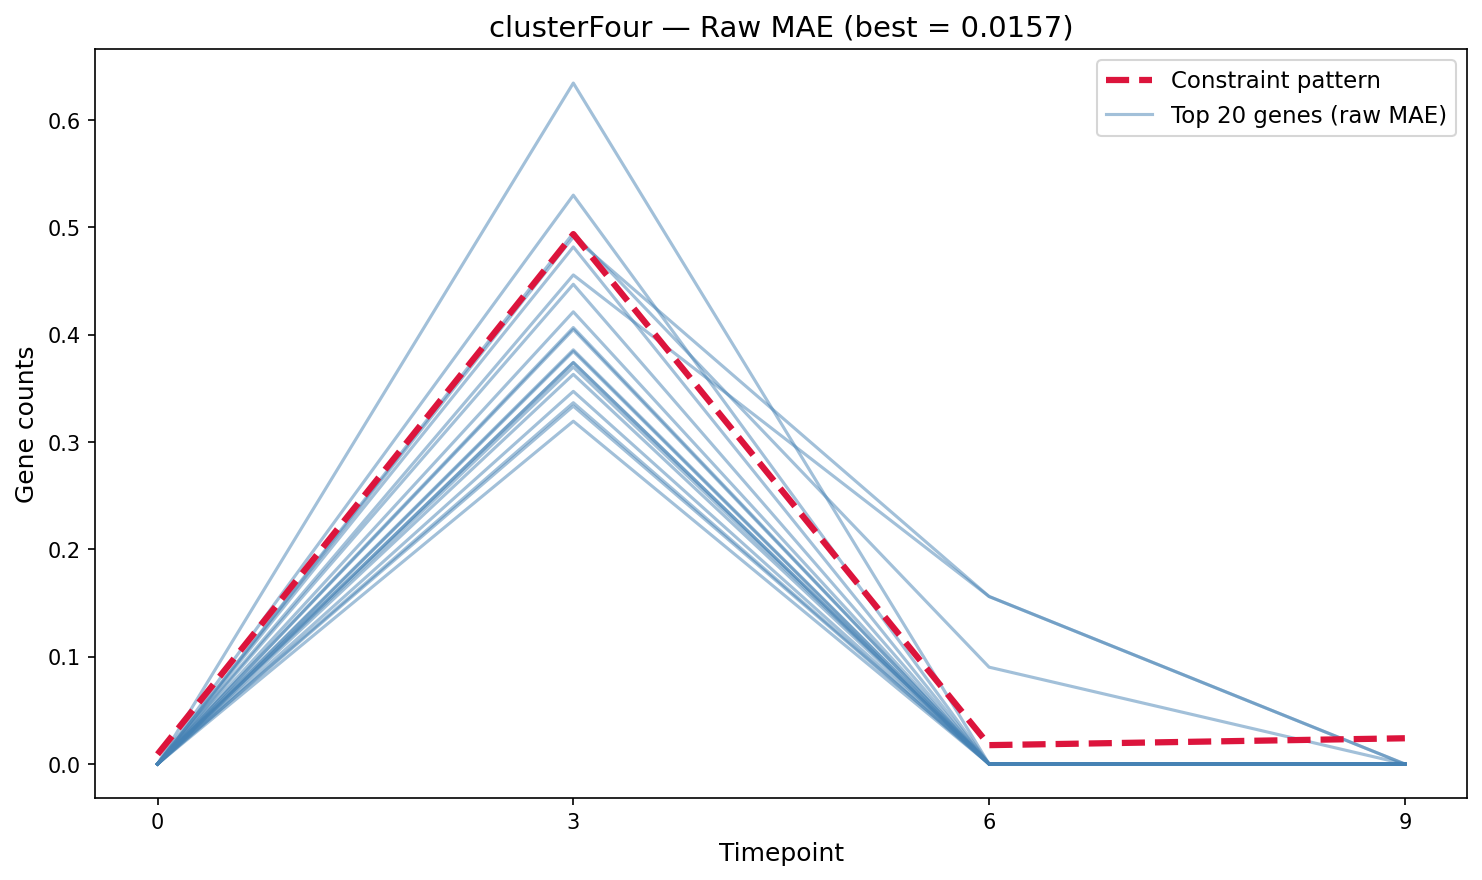
\includegraphics[width=\textwidth]{plots/rawmae_clusterFour.png}
\end{column}
\begin{column}{0.36\textwidth}
\vspace{1em}
\textbf{For the first time}, genes actually follow the spike pattern.\\[0.5em]
0/20 overlap with any original method --- none of them found these genes because normalization erased the magnitude.
\end{column}
\end{columns}
\end{frame}

% ------------------------------------------------------------------
\begin{frame}{Raw MAE: clusterOne}
\begin{columns}[T]
\begin{column}{0.62\textwidth}
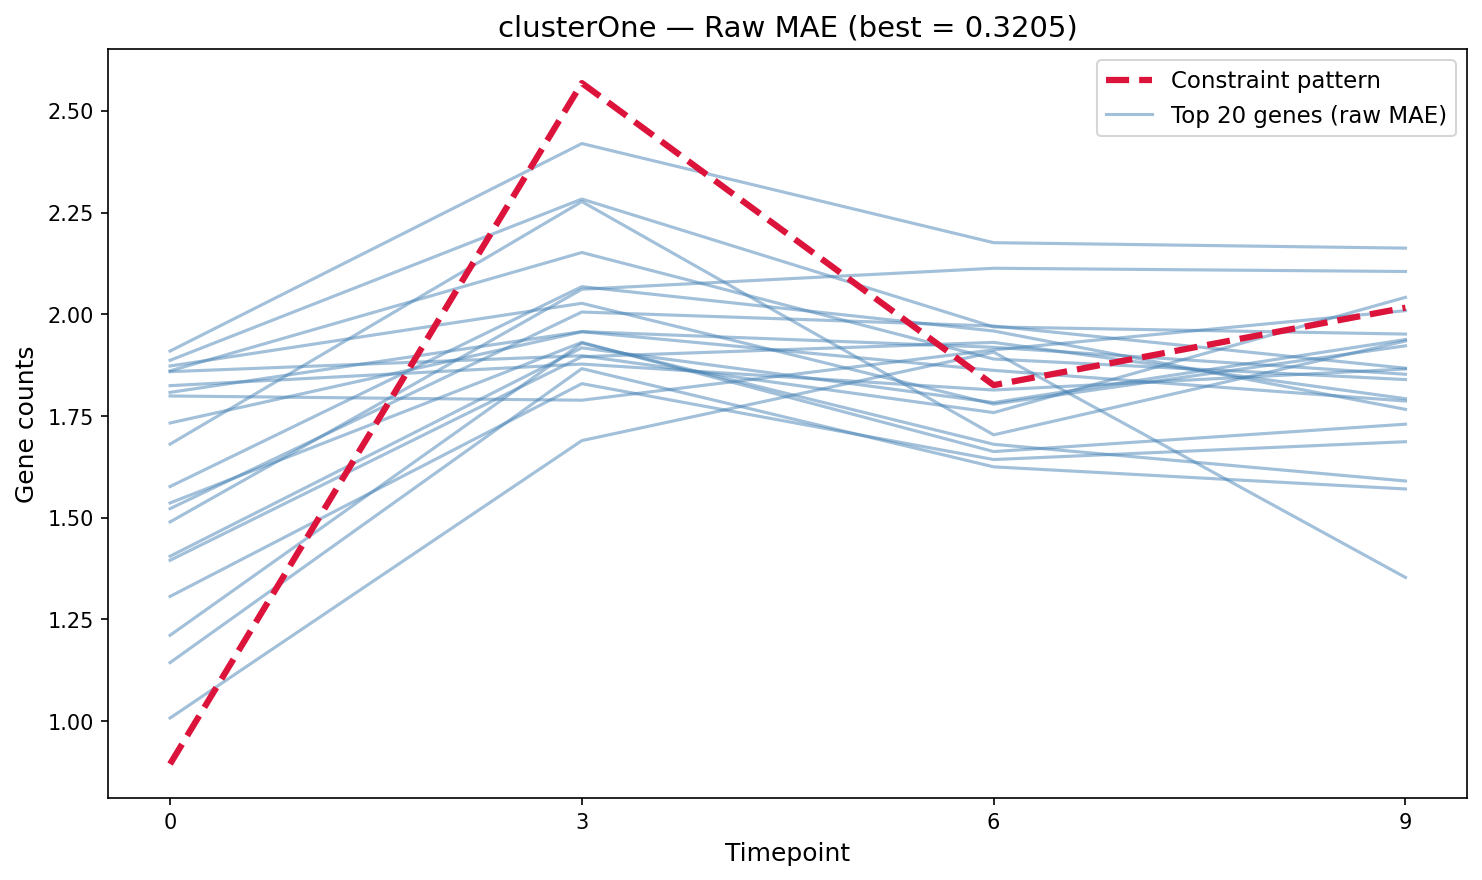
\includegraphics[width=\textwidth]{plots/rawmae_clusterOne.png}
\end{column}
\begin{column}{0.36\textwidth}
\vspace{1em}
The exception --- genes at the pattern's magnitude don't follow the spike shape.\\[0.5em]
For this cluster, the shape-based methods may be more appropriate.\\[0.5em]
\textbf{Raw MAE isn't always better} --- it depends on what the pattern looks like.
\end{column}
\end{columns}
\end{frame}

% ------------------------------------------------------------------
\begin{frame}{Discussion}
\begin{itemize}\itemsep8pt
  \item \textbf{Raw MAE} gives the best visual fit for clusters Two, Three, and Four
  \item \textbf{clusterOne} is the exception --- genes at the pattern's magnitude\\
        don't follow its shape. Shape-based methods do better here.
  \item \textbf{Key insight:} all 6 original methods operate on normalized data,\\
        which erases magnitude. This is why they find genes with\\
        the right shape but at the wrong expression level.
  \item \textbf{Open question:} is matching the exact expression level biologically\\
        meaningful, or is shape similarity sufficient?\\
        If expression level matters $\rightarrow$ raw MAE on unnormalized data.\\
        If only the temporal shape matters $\rightarrow$ the normalized methods\\
        (Pearson, DTW, etc.) with gating may be more appropriate.
\end{itemize}
\end{frame}

\end{document}
